\section{Technically speaking}
\mode<presentation>{
	\begin{frame}
	\frametitle{Technically speaking}
	\begin{itemize}
		\item<1-> SystemC is an IEEE standard (IEEE 1666) C++ class library for system and hardware design.
		\item<1-> The standard has been proposed and is maintained by the \emph{Open SystemC Initiative} (OSCI).
		\item<1-> The SystemC Library provides provides constructs missing in standard C++ necessary to model system architecture:
		\begin{itemize}
			\item<1-> hardware timing
			\item<1-> concurrency
			\item<1-> reactive behavior
		\end{itemize}
	\end{itemize}
\end{frame}
}

\mode<article>{
As mentioned previously, SystemC is a C++ class library for system and hardware design, that has been standardized by the IEEE: IEEE 1666. 
The standard has been proposed and it is maintained by the \emph{Open SystemC Initiative} (OSCI).
SystemC is often thought of as a hardware description language like VHDL and Verilog, but is more aptly described as a system description language, since it exhibits its real power during \emph{transaction-level modeling} and \emph{behavioral modeling}.
SystemC is a set of library routines and macros implemented in C++, which makes it possible to simulate {concurrent processes}, each described by ordinary C++ syntax. 
Instantiated in the SystemC framework, the objects described in this manner may communicate in a simulated real-time environment, using signals of all the datatypes offered by C++, some additional ones offered by the SystemC library, as well as user defined.

A reference (and free) implementation of the SystemC library is provided by the OSCI consortium.
Other implementations (or partial implementations) are available and most of them are commercial products.
In this tutorial we will work with the reference implementation.
}

\subsection{Installing OSCI SystemC (under Linux)}

\mode<presentation>{
\begin{frame}
	\frametitle{Installing OSCI SystemC\newline Download}
	\begin{itemize}
		\item<1-> The SystemC reference implementation can be downloaded from the OSCI website:
		\begin{itemize}
			\item<1-> http://www.systemc.org
			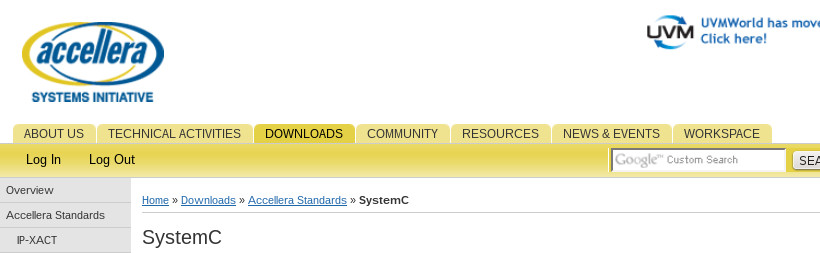
\includegraphics[width=0.6\textwidth]{introduction/figures/osci_homepage.jpg}
		\end{itemize}
		\item<1-> To download SystemC you will have to register yourself into the OSCI website.
		\item<1-> From the same site you can download:
		\begin{itemize}
			\item<1-> reference manuals and documents,
			\item<1-> new SystemC proposals and standards, like the recently proposed TLM2.0 proposal.
		\end{itemize}
	\end{itemize}
\end{frame}

\begin{frame}
	\frametitle{Installing OSCI SystemC\newline Compile \& Install}
	\begin{itemize}
		\item<1-> Uncompress the downloaded file.
		\item<1-> Create a directory for the compilation and a directory to install the final library.
		\item<1-> Into the compilation directory perform the typical \texttt{configure}, \texttt{make} and \texttt{make install} to install the SystemC library.
	\end{itemize}
	\lstinputlisting[language= ,basicstyle=\ttfamily\tiny,numbers=none,breaklines=true,framexleftmargin=0.5mm,xleftmargin=0.06\textwidth,xrightmargin=0.06\textwidth]{introduction/install.txt}
\end{frame}
}

\mode<article>{
To install SystemC you will have to download it from the OSCI SystemC site: http://www.systemc.org~.
To do so you will have to register yourself into the OSCI site.
From the same site you can download other documents, manuals and the new proposals like the TLM2.0 proposal.

Once you have downloaded the SystemC compressed file you have to simply uncompress it and follow the indications that appear in the INSTALL file.
Those instructions will depend on the operating system you use.
Currently SystemC can be install under Windows, Linux and MacOSX among others.

Under Linux you will have to create a directory were SystemC will be compiled (we will call it \texttt{obj} for our example). 
From the \texttt{obj} directory you will have to call the \texttt{configure} script available from the downloaded SystemC distribution (see Figure~\ref{technically_systemc_configure}). 
The \texttt{configure} script accepts different options but usually you will be only using the \texttt{--prefix} option, which defines in which directory the SystemC library will be installed.
Note that the installation directory needs to be created before performing the following step.
Once the \texttt{configure} script has finished its task, you can perform the typical\footnote{At least typical for  many Linux users.} \texttt{make} and \texttt{make install} to compile and install the SystemC library\footnote{If you selected as install directory a directory that belongs to another user, for example the root user, you will have to perform the \texttt{make install} step under that user.}.

\begin{figure}[!h]
\begin{center}
		\lstinputlisting[language= ,basicstyle=\ttfamily\normalsize,numbers=none,breaklines=true,framexleftmargin=0.5mm,xleftmargin=0.06\textwidth,xrightmargin=0.06\textwidth]{introduction/install.txt}
\end{center}
\label{technically_systemc_configure}
\caption{Commands to install SystemC (exemple).}
\end{figure}

Now you can develop simulators based on SystemC using your newly installed library.
When creating your simulators you will have to include the \texttt{systemc.h} header file that you can find in the \texttt{include} directory of your installation. 
When compiling you will have to define the location of the SystemC headers directory and precise that you are using the SystemC library and its location (the \texttt{lib-linux} directory).
}

